% D.13 △ABC 中 DE∥BC，两部分面积之比 4:5
\documentclass[tikz,border=4pt]{standalone}
\usepackage{ctex}
\usepackage{amsmath}
\usetikzlibrary{calc}
\begin{document}
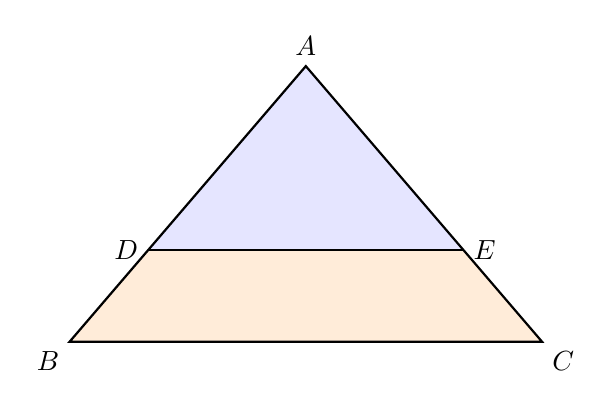
\begin{tikzpicture}[scale=1.0, thick]
  \coordinate (A) at (1, 3.5);
  \coordinate (B) at (-2, 0);
  \coordinate (C) at (4, 0);
  % AD:AB = 2:3（面积比 4:9，上小下大 4:5）
  \coordinate (D) at ($(A)!0.667!(B)$);
  \coordinate (E) at ($(A)!0.667!(C)$);

  \fill[blue!10] (A) -- (D) -- (E) -- cycle;
  \fill[orange!15] (D) -- (B) -- (C) -- (E) -- cycle;

  \draw (A) -- (B) -- (C) -- cycle;
  \draw (D) -- (E);

  \node[above]       at (A) {$A$};
  \node[below left]  at (B) {$B$};
  \node[below right] at (C) {$C$};
  \node[left]        at (D) {$D$};
  \node[right]       at (E) {$E$};
\end{tikzpicture}
\end{document}
